\documentclass[border=15pt, multi, tikz]{standalone}
\usepackage{import}
\subimport{./layers/}{init}
\usetikzlibrary{positioning}
\usetikzlibrary{3d} %for including external image 

\def\ConvColor{rgb:yellow,5;red,2.5;white,5}
\def\ConvReluColor{rgb:yellow,5;red,5;white,5}
\def\PoolColor{rgb:red,1;black,0.3}
\def\DcnvColor{rgb:blue,5;green,2.5;white,5}
\def\SoftmaxColor{rgb:magenta,5;black,7}
\def\SumColor{rgb:blue,5;green,15}

\begin{document}
\begin{tikzpicture}
\tikzstyle{connection}=[ultra thick,every node/.style={sloped,allow upside down},draw=\edgecolor,opacity=0.7]
%%%%%%%%%%%%%%%%%%%%%%%%%%%%%%%%%%%%%%%%%%%%%%%%%%%%%%%%%%%%%%%%%%%%%%%%%%%%%%%%%%%%%%%%
%% Draw Layer Blocks
%%%%%%%%%%%%%%%%%%%%%%%%%%%%%%%%%%%%%%%%%%%%%%%%%%%%%%%%%%%%%%%%%%%%%%%%%%%%%%%%%%%%%%%%
\node[canvas is zy plane at x=0] (temp) at (-2,0,0) {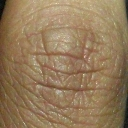
\includegraphics[width=5cm,height=5cm]{finger-knuckle.jpg}};
% conv1_1,conv1_2
\pic[shift={(0,0,0)}] at (0,0,0) {RightBandedBox={name=cr1,caption=conv1,%
        xlabel={{"32","32"}},zlabel=I/2,fill=\ConvColor,bandfill=\ConvReluColor,%
        height=20,width=2,depth=20}};

% conv2_1,conv2_2
\pic[shift={(0.8,0,0)}] at (cr1-east) {RightBandedBox={name=cr2,caption=conv2,%
        xlabel={{"64", "64"}},zlabel=I/4,fill=\ConvColor,bandfill=\ConvReluColor,%
        height=17,width={4},depth=17}};

% conv3_1,conv3_2
\pic[shift={(1,0,0)}] at (cr2-east) {RightBandedBox={name=cr3,caption=conv3,%
        xlabel={{"128","128","128"}},zlabel=I/4,fill=\ConvColor,bandfill=\ConvReluColor,%
        height=17,width={8},depth=17}};

% resid1
\pic[shift={(1.5,0,0)}] at (cr3-east) {RightBandedBox={name=res1,caption=res1,%
        xlabel={{"128","128","128"}},zlabel=I/4,fill=\ConvColor,bandfill=\ConvReluColor,%
        height=17,width={7, 7},depth=17}};

\pic[shift={(1.5,-6,0)}] at (cr3-east) {Box={name=rescr3,%
        xlabel={{"128","128","128"}},zlabel=I/4,fill=\ConvColor,%
        height=17,width={8},depth=17}};

\pic[shift={(1,0,0)}] at (res1-east) {Ball={name=elt1,%
        fill=\SumColor,opacity=0.6,%
        radius=2.5,logo=$+$}};

% resid2
% conv5_1, conv5_2
\pic[shift={(1,0,0)}] at (elt1-east) {RightBandedBox={name=res2,caption=res2,%
        xlabel={{"128","128","128"}},zlabel=I/4,fill=\ConvColor,bandfill=\ConvReluColor,%
        height=17,width={7, 7},depth=17}};

\pic[shift={(1.5,5.5,0)}] at (elt1-east) {Box={name=resres1,%
        xlabel={{"128","128","128"}},zlabel=I/4,fill=\ConvColor,%
        height=17,width={8},depth=17}};

\pic[shift={(1,0,0)}] at (res2-east) {Ball={name=elt2,%
        fill=\SumColor,opacity=0.6,%
        radius=2.5,logo=$+$}};

% resid3
% conv6_1, conv6_2
\pic[shift={(1,0,0)}] at (elt2-east) {RightBandedBox={name=res3,caption=res3,%
        xlabel={{"128","128","128"}},zlabel=I/4,fill=\ConvColor,bandfill=\ConvReluColor,%
        height=17,width={7, 7},depth=17}};

\pic[shift={(1.5,-6,0)}] at (elt2-east) {Box={name=resres2,%
        xlabel={{"128","128","128"}},zlabel=I/4,fill=\ConvColor,%
        height=17,width={8},depth=17}};

\pic[shift={(1,0,0)}] at (res3-east) {Ball={name=elt3,%
        fill=\SumColor,opacity=0.6,%
        radius=2.5,logo=$+$}};

% resid4
% conv7_1, conv7_2
\pic[shift={(1,0,0)}] at (elt3-east) {RightBandedBox={name=res4,caption=res4,%
        xlabel={{"128","128","128"}},zlabel=I/4,fill=\ConvColor,bandfill=\ConvReluColor,%
        height=17,width={7, 7},depth=17}};

\pic[shift={(1.5,5.5,0)}] at (elt3-east) {Box={name=resres3,%
        xlabel={{"128","128","128"}},zlabel=I/4,fill=\ConvColor,%
        height=17,width={8},depth=17}};

\pic[shift={(1,0,0)}] at (res4-east) {Ball={name=elt4,%
        fill=\SumColor,opacity=0.6,%
        radius=2.5,logo=$+$}};

% conv4_1,conv4_2
\pic[shift={(1,0,0)}] at (elt4-east) {RightBandedBox={name=cr4,caption=conv4,%
        xlabel={{"64","64"}},zlabel=I/4,fill=\ConvColor,bandfill=\ConvReluColor,%
        height=17,width=4,depth=17}};

% conv5_1, conv5_2       
\pic[shift={(1,0,0)}] at (cr4-east) {RightBandedBox={name=cr5,caption=conv5,%
xlabel={{"1","64"}},zlabel=I/4,fill=\DcnvColor,%
height=17,width=1,depth=17}};

\node[canvas is zy plane at x=0] (temp) at (30,0,0) {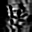
\includegraphics[width=3cm,height=3cm]{feature.png}};


%%%%%%%%%%%%%%%%%%%%%%%%%%%%%%%%%%%%%%%%%%%%%%%%%%%%%%%%%%%%%%%%%%%%%%%%%%%%%%%%%%%%%%%%
%% Draw connections
%%%%%%%%%%%%%%%%%%%%%%%%%%%%%%%%%%%%%%%%%%%%%%%%%%%%%%%%%%%%%%%%%%%%%%%%%%%%%%%%%%%%%%%%
\draw [connection]  (0,0,0)    -- node {\midarrow} (cr2-west);
\draw [connection]  (cr2-east)    -- node {\midarrow} (cr3-west);
\draw [connection]  (cr3-east)    -- node {\midarrow} (res1-west);
\draw [connection]  (res1-east)    -- node {\midarrow} (elt1-west);
\draw [connection]  (elt1-east)    -- node {\midarrow} (res2-west);
\draw [connection]  (res2-east)    -- node {\midarrow} (elt2-west);
\draw [connection]  (elt2-east)    -- node {\midarrow} (res3-west);
\draw [connection]  (res3-east)    -- node {\midarrow} (elt3-west);
\draw [connection]  (elt3-east)    -- node {\midarrow} (res4-west);
\draw [connection]  (res4-east)    -- node {\midarrow} (elt4-west);
\draw [connection]  (elt4-east)    -- node {\midarrow} (cr4-west);
\draw [connection]  (cr4-east)    -- node {\midarrow} (cr5-west);


%% Skip connections
\path (cr3-east) -- (res1-west) coordinate[pos=0.25] (between3_4) ;
\draw [connection]  (between3_4)    -- node {\midarrow} (rescr3-west-|between3_4) -- node {\midarrow} (rescr3-west);
\draw [connection]  (rescr3-east) -- node {\midarrow} (rescr3-east -| elt1-south) -- node {\midarrow} (elt1-south);

\path (elt1-east) -- (res2-west) coordinate[pos=0.25] (between4_5) ;
\draw [connection]  (between4_5)    -- node {\midarrow} (resres1-west-|between4_5) -- node {\midarrow} (resres1-west);
\draw [connection]  (resres1-east) -- node {\midarrow} (resres1-east -| elt2-north) -- node {\midarrow} (elt2-north);

\path (elt2-east) -- (res3-west) coordinate[pos=0.25] (between5_6) ;
\draw [connection]  (between5_6)    -- node {\midarrow} (resres2-west-|between5_6) -- node {\midarrow} (resres2-west);
\draw [connection]  (resres2-east) -- node {\midarrow} (resres2-east -| elt3-south) -- node {\midarrow} (elt3-south);

\path (elt3-east) -- (res4-west) coordinate[pos=0.25] (between6_7) ;
\draw [connection]  (between6_7)    -- node {\midarrow} (resres3-west-|between6_7) -- node {\midarrow} (resres3-west);
\draw [connection]  (resres3-east) -- node {\midarrow} (resres3-east -| elt4-north) -- node {\midarrow} (elt4-north);


\end{tikzpicture}
\end{document}\grid
